\documentclass[letterpaper,10pt,twocolumn]{article}
%\usepackage{natbib}
%\bibpunct{[}{]}{,}{a}{}{;}
\let\citep\cite
\let\citeyear\cite
\let\citeyearpar\cite
\usepackage{usenix}
%\usepackage{endnotes}
%\let\footnote\endnote
\let\theendnotes\relax

\usepackage{amsmath}
\usepackage{graphicx}
\usepackage{xspace}
\usepackage[hyphens]{url}
\usepackage{extensions}
\usepackage{microtype}
\usepackage[T1]{fontenc}
\usepackage{textcomp}
\usepackage[scaled=0.85]{beramono}
\usepackage{ifthen}
\usepackage{alltt}
\usepackage[format=hang,indention=0cm]{subcaption}
\usepackage{fixltx2e}
\usepackage{tikz}
\usetikzlibrary[fit,backgrounds,calc,chains,matrix,positioning,scopes,arrows,decorations,decorations.markings]
% The sigplanconf document class uses hoffset and voffset to set
% margins.  This is a poor way to do it, and it causes problems with
% eso-pic.  This hack fixes things.
\usepackage[final,nofancy,notoday]{svninfo}
% \makeatletter
% \if@svnInfoDraft@
%   \usepackage{eso-pic}
%   \newlength{\msgX}\setlength{\msgX}{5pt}\addtolength{\msgX}{-\hoffset}
%   \newlength{\msgY}\setlength{\msgY}{5pt}\addtolength{\msgY}{\voffset}
%   \AddToShipoutPicture{%
%     \setlength{\unitlength}{1mm}%
%     \put(\LenToUnit{\the\msgX},\LenToUnit{\the\msgY}){\tiny\svnInfoFile\quad\svnInfoRevision\quad\svnInfoDate%
%       \quad\svnInfoTime\quad\svnInfoOwner}%
%   }
% \fi
% \makeatother

%\usepackage{setspace}
%\usepackage{rotating}
%\usepackage{ragged2e}



\usepackage[implicit=true,%
            bookmarks=false,%
            bookmarksopen=false,%
            pdfpagemode=UseNone,%
            colorlinks=false,%
            pdfborder={0 0 0},%
            plainpages=false,%
            pdfpagelabels=true,%
            pdfpagelayout=SinglePage]{hyperref}
\usepackage[capitalize]{cleveref}

\usepackage{enumitem}
\newlist{compactitem}{itemize}{3}
\setlist[compactitem]{
  topsep=0\baselineskip plus 0.5\baselineskip,
  partopsep=0pt,
  itemsep=0\baselineskip plus 0.5\baselineskip,
  parsep=0pt,
  label=\textbullet
}
\newlist{compactdesc}{description}{3}
\setlist[compactdesc]{
  topsep=0\baselineskip plus 0.5\baselineskip,
  partopsep=0pt,
  itemsep=0\baselineskip plus 0.5\baselineskip,
  parsep=0pt,
}
\newlist{compactenum}{enumerate}{3}
\setlist[compactenum]{
  topsep=0.25\baselineskip plus 0.25\baselineskip minus 0.25\baselineskip,
  partopsep=0pt,
  itemsep=0.25\baselineskip plus 0.25\baselineskip minus 0.25\baselineskip,
  parsep=0pt,
  label={\arabic*.},ref={\arabic*}
}


\makeatletter
\newcommand{\paraemph}{\@startsection{paragraph}{4}{\z@}%
  {3.25ex \@plus 1ex \@minus .2ex}{-1em}{\normalfont\normalsize\itshape}}
\newcommand{\quot}{\mbox{\tt\char'042}}
\newcommand{\wild}{\mbox{\tt\char'137}}
\newcommand{\impl}[1]{{\def\_{\wild}\def\"{\quot}\tt#1}}
\newcommand{\mimpl}[1]{\text{\impl{#1}}}
\newcommand{\code}[1]{{\def\"{\quot}\ensuremath{\mathsf{#1}}}}
\newcommand{\meta}[1]{{\def\"{\quot}\ensuremath{\mathrm{#1}}}}
\newcommand{\kw}[1]{\ensuremath{\langle\mathit{#1}\rangle}}
\newcommand{\setOf}[1]{\ensuremath{\left\lbrace#1\right\rbrace}}
\usepackage{pifont}
\newcommand{\CR}{\Pisymbol{psy}{191}}
\DeclareRobustCommand{\spec}[1]{\textsf{#1}\xspace}
\let\oldC=\C
\DeclareRobustCommand\C{\@ifnextchar3\myC\CSharp}
\DeclareRobustCommand\myC[1]{\spec{C3}}
\DeclareRobustCommand\CSharp[1]{\ifthenelse{\equal{#1}{\#}}{\spec{C\textsuperscript{\#}}}{\oldC}}
\DeclareRobustCommand\JS{\spec{JS}}
\DeclareRobustCommand\CSS{\@ifnextchar2{\CSSTwo}{\@ifnextchar3{\CSSThree}{\spec{CSS}}}}
\DeclareRobustCommand\CSSTwo[1]{\@ifnextchar.{\CSSTwoDot}{\spec{CSS\,2}}}
\DeclareRobustCommand\CSSTwoDot[1]{\@ifnextchar1{\CSSTwoDotOne}{\spec{CSS\,2}}}
\DeclareRobustCommand\CSSTwoDotOne[1]{\spec{CSS\,2.1}}
\DeclareRobustCommand\CSSThree[1]{\spec{CSS\,3}}
\DeclareRobustCommand\XBL{\@ifnextchar1{\XBLOne}{\@ifnextchar2{\XBLTwo}{\spec{XBL}}}}
\DeclareRobustCommand\XBLOne[1]{\spec{XBL\,1}}
\DeclareRobustCommand\XBLTwo[1]{\spec{XBL\,2.0}}
\DeclareRobustCommand\XML{\spec{XML}}
\DeclareRobustCommand\XUL{\spec{XUL}}
\DeclareRobustCommand\ECMAScript{\@ifnextchar3{\ECMAScriptThree}{\@ifnextchar5{\ECMAScriptFive}{\spec{ECMAScript}}}}
\DeclareRobustCommand\ECMAScriptFive[1]{\spec{ECMAScript\,5}}
\DeclareRobustCommand\HTML{\@ifnextchar4{\HTMLFour}{\@ifnextchar5{\HTMLFive}{\spec{HTML}}}}
\DeclareRobustCommand\HTMLFive[1]{\spec{HTML\,5}}
\DeclareRobustCommand\HTMLFour[1]{\@ifnextchar.{\HTMLFourDot}{\spec{HTML\,4}}}
\DeclareRobustCommand\HTMLFourDot[1]{\@ifnextchar0{\HTMLFourDotOh}{\spec{HTML\,4}.}}
\DeclareRobustCommand\HTMLFourDotOh[1]{\@ifnextchar1{\HTMLFourDotOhOne}{\spec{HTML\,4.0}}}
\DeclareRobustCommand\HTMLFourDotOhOne[1]{\spec{HTML\,4.01}}
\makeatother

\DeclareRobustCommand{\LJS}{\ensuremath{\lambda_\JS}\xspace}
\usepackage{lipsum}
\begin{document}

\date{}

\title{Featherweight DOM Events}
\def\and{\hskip 1em}
\author{%
{\rm Matt Carroll \and Hannah Quay-de la Vallee \and Dan Kimmel}\\%
{\rm Benjamin S. Lerner \and Shriram Krishnamurthi}\\%
Brown University%
}
\maketitle

%\thispagestyle{empty}

\begin{abstract}
  \lipsum[1]
\end{abstract}

\section{Introduction}\label{sec:introduction}
Modern web applications are fluid collections of script and markup
that respond and adapt to user interaction.  Because their programming
model differs from classic desktop applications, the \emph{analysis}
of such programs is still in its infancy.  To date, most efforts have
focused on individual portions in isolation: huge progress has been
made in clarifying the semantics of \JS [CITECITECITE], in modeling
the tree structure of \HTML [CITECITECITE], and in understanding the
overall behavior of the browser as a runtime environment
[CITECITECITE].  But each of these approaches ignores the crucial
element of reactivity: web programming is fundamentally
\emph{event-driven}, and employs a powerful mechanism for event
propagation.  Perhaps counterintuitively, the \JS loaded in web
applications is largely \emph{inert}, and only executes when triggered
by events dispatching through the \HTML structure in which it resides.
To paraphrase Alan Guth's famous dictum, ``\HTML tells events how to
propagate, and events tell \HTML how to evolve.''

The ability to model web applications more accurately has widespread
appeal.  Webapps are large codebases in languages with (currently)
poor support for modularity: how can we assure ourselves that a
program doesn't exhibit unintended behaviors?  Many webapps include
semi- or untrusted content such as ads: how can we ensure that a
program is robust in the face of the injected content's activity?  And
for many web-like applications, foremost among them Firefox or
Thunderbird, users avidly install extensions that deliberately and
deeply modify the markup and script of the underlying program: what
assurance do we have that the composite program will work correctly?
Even those current tools which do attempt to model both the page
structure and the code [CITECITECITE] are hampered by state-space
explosion, as without a precise model the potential code paths grow
beyond feasibility.

Instead, we propose a simple, executable, testable model of event
dispatch in web applications, in the style of \LJS
[CITECITECITE].  Our model is engineered to hew closely to the
structure of the spec [CITE], to build confidence in the model's
adequacy.  For our purposes we abstract \JS and model only those APIs
dealing with page structure or events; the model is easily extended to
include \LJS directly.  Likewise we represent the page
structure as a simple tree in a heap; again the model can be extended
with a richer tree representation [CITECITE] for further precision.


\subsection{Contributions}
Specifically, this paper provides the following contributions:
\begin{enumerate}
\item A short, executable, and testable model of event dispatch.
  Writing such a model clarifies potential sources of confusion in the
  spec itself, provides an oracle against which implementations can be
  tested, and provides a foundation for future program analyses.  As a
  case in point, systematically testing small examples in our model
  revealed discrepant behavior among the major browsers.
\item Simple proofs that the model upholds properties expected of the
  spec, such as precisely how and when script's side effects can
  affect the dipatching of current and subsequent events.  Because the
  model closely resembles the spec, such proofs lend confidence that
  the spec itself enjoys the same properties; thus far such claims
  were merely the \emph{intent} of the lengthy, prose spec.
\item An application of the model to ADsafe [CITE], to determine
  whether ADsafe widgets in fact may still affect the control flow of
  their host, despite the ADsafe sandbox.
\item An application of the model to two Thunderbird extensions to
  detect a real conflict between them.  Further, the model is used to
  show that the fix (as implemented by one extension author)
  currently suffices to correct the bug, but that another, simpler fix
  is more robust.
\end{enumerate}
Elaborating our model into a fully-fledged testing tool or model
checker, which can scale to full-size programs, is an engineering
effort left to future work.

\section{Understanding web program control flow}\label{sec:c3-architecture}
The intuitive but incomplete model for programming web pages is that
of an asynchronous event loop, where events are triggered by user
interaction, and with event callbacks that have access to an object
graph representing the tree structure of the \HTML, known as the
Document Object Model (DOM).  The full definition of ``the DOM'' is in
fact spread over many specifications [CITECITECITECITECITE],
comprising far more than just this tree structure.  In reality, the
DOM object graph is more interconnected than a mere tree and can be
arbitrarily entangled with the \JS heap; event callbacks are attached
directly to these DOM nodes; and while the event loop itself is not
available as a first-class entity through the DOM, nodes may support
APIs that implicitly cause further events to be dispatched or that
modify the tree structure.

In short, it is na\"{\i}ve to think of the execution of a web program
as merely an event loop alongside a tree-structured data store.
Rather, the structure of the tree influences the propagation of
events, and the side effects of events can modify the tree.
Understanding web program behavior therefore requires modeling all the
subtleties of event dispatch through the DOM.  Like all portions of
web-related programming, the event mechanisms were developed over
time, resulting in historical quirks and oddities.  We explain the
main features of event dispatch in this section, then develop our
model of it in the following one.

\subsection{Event dispatch in $N$ easy stages}
\paragraph{Static document structure, one event listener}
We take as a running example a simple document fragment of three
nodes: \ftag{div}{}{\ftag{p}{}{\stag{span}}}.  In the simplest case,
suppose as the page loads we attach a single event listener to the
\stag{span}:
\begin{alltt}
  spanNode.addEventListener("click",
    function(event) \{ alert("In click"); \});
\end{alltt}

This statement registers the function as an \emph{listener} for mouse
``click'' events only; any other event types are ignored.  When an
event is \emph{dispatched} to a particular \emph{target}, the
listener on that target for that event type---if there is one---is
invoked.  Thus a ``click'' event targeted at the \stag{span} will
yield the alert; a ``keypress'' event will not, nor will a ``click''
event targeted at the \stag{p} node.

Note that scripts can construct new event objects programmatically and
then dispatch them to target nodes.  These events behave identically
to browser-generated events, with one caveat addressed later.
\paragraph{Multiple listeners and the dispatch chain}
The above example is unnecessarily restricted in two key ways.  First,
the suggestively named \impl{addEventListener} API can in fact be used
repeatedly, for the same node and the same event type, to add
\emph{multiple} listeners for an event.  These listeners will be
called in the order they were installed whenever their triggering
event is dispatched.  This flexibiility allows for cleaner program
structure: clicking on a form button, say, might trigger both the
display of new form fields and the validation of existing ones; these
disparate pieces of functionality can now be in separate listeners
rather than one monolithic one.

Second, web programs frequently may respond to events on several
elements in the same way.  One approach would be to install the same
function as a listener on each such element, but this is brittle if
the page structure is later changed.  Instead, a more robust approach
would install the listener once on the nearest common ancestor of all
the intended targets.  To achieve this, event dispatch will call
listeners on \emph{each ancestor of the target node} as well, known as
the \emph{dispatch chain}.  Thus adding a listener to the other two
nodes in our example:
\begin{alltt}
  function listener(event) \{
    alert("At " + event.currentTarget.nodeName +
          " with actual target " + 
          event.target.nodeName);
  \}
  pNode.addEventListener("click", listener);
  divNode.addEventListener("click", listener);
\end{alltt}
will trigger \emph{three} alerts: ``In click'', ``At p with actual
target span'', and ``At div with actual target span'' in that order:
the event ``bubbles'' from the target node through its
ancestors to the root of the document.\footnote{Additionally, for
  legacy reasons it also propagates to the global \impl{window}
  object; this detail does not substantially change any of our
  subsequent modeling.}

For symmetry, programs may want to perform some generic response
\emph{before} the event reaches the target node, rather than only
after.  Accordingly, event dispatch in fact defines a so-called
\emph{capturing} phase, where listeners are called starting at the
root and propagating down to the target node.  To install a
capture-phase listener, \impl{addEventListener} takes a third, boolean
\impl{useCapture} parameter: when true, the listener is for capturing;
when missing or false, the listener is for bubbling.

Event dispatch therefore comprises three phases: ``capture'', from
root to the target's parent and running only capture-phase listeners;
``target'', at the target node and running all listeners; and
``bubble'', from the target's parent to the root and running only
bubble-phase listeners.  The \impl{event} parameter to each listener
contains three fields indicating the current \impl{eventPhase}, the
\impl{currentTarget}, and the intended \impl{target} of the event.
For our running example, an event targeted at the \stag{span} will
call listeners
\begin{compactenum}
\item On \stag{div} for phase \impl{capture}, then
\item On \stag{p} for phase \impl{capture}, then
\item On \stag{span} for phase \impl{target}, then
\item On \stag{p} for phase \impl{bubble}, then
\item On \stag{div} for phase \impl{bubble}.
\end{compactenum}
\paragraph{Aborting event propagation}
It may be the case that a capture- or target-phase listener completely
handles an event, and that the app has no need to propagate the event
further.  The app could maintain some global flag and have each
listener check the flag and abort accordingly, but this is tedious and
error-prone.  Instead, the \impl{event} object can be used to stop the
event propagation in two ways:
\begin{compactitem}
\item \impl{event.stopPropagation()} tells dispatch to terminate as
  soon as all listeners on the current node complete, regardless of
  whether listeners are installed on future nodes of the dispatch
  chain.  Thus calling this in a target-phase listener on \stag{span}
  will abort dispatch between steps~3 and~4 above.
\item \impl{event.stopImmediatePropagation()} tells dispatch to
  terminate as soon as the current listener returns, regardless of
  whether other listeners are installed on this or future nodes in the
  dispatch chain.  Thus calling this in a capture-phase listener on
  \stag{p} will abort dispatch in the middle of step~2, even if there
  are more capture-phase listeners on \stag{p}.
\end{compactitem}

\paragraph{Dynamic document structure: no effect!}
So far our example listeners have had no side effects; in general,
however, they often do.  This may interact oddly with the informal
definitions above: for instance, if a target-phase listener removes
the target node from the document, what should the dispatch chain be?
Several options are possible; the currently specified behavior is that
the dispatch chain is \emph{fixed} at the beginning of dispatch, and
is unmodified by changes in document structure.  Thus in our running
example, regardless of whether nodes are deleted, re-parented or
otherwise modified, the five steps listed are unaffected.

\paragraph{Dynamic listeners: some effect!}
We can now address the last oversimplification, that event listeners
are added once and for all at the start of the program.  In fact they
can be added and removed dynamically (using the analogous
\impl{removeEventListener} API) throughout the program's execution.
For example, a common idiom is the ``run-once'' listener that removes
itself the first time it runs:
\begin{alltt}
  function runOnce(event) \{
    targetNode.removeEventListener("click", runOnce);
    ...
  \}
  targetNode.addEventListener("click", runOnce);
\end{alltt}

Such actions have a limited effect on the current dispatch: listeners
added (resp. removed) to a \emph{future} node in the dispatch chain
will (resp. will not) be called by the dispatch algorithm; listeners
added (resp. removed) to the \emph{current} or \emph{past} nodes in
the dispatch chain will be ignored (resp. will still be called).  More
intuitively, a refinement of the five steps above says that 
dispatching an event to \stag{span} will:
\begin{compactitem}
\item Determine the capture-phase listeners on \stag{div} and run
  them, then
\item Determine the capture-phase listeners on \stag{p} and run
  them, then
\item Determine the target-phase (i.e. all) listeners on \stag{span} and run
  them, then
\item Determine the bubble-phase listeners on \stag{p} and run
  them, then
\item Determine the bubble-phase listeners on \stag{div} and run
  them.
\end{compactitem}
Since the determination of the relevant listeners is lazily computed
in each step, dispatch will only notice added or removed listeners
that apply to later steps.

\paragraph{Dealing with legacy ``handlers''}
Unfortunately, the mechanism explained so far---multiple listeners,
capturing and bubbling, and cancellation---was not the first model
proposed.  Originally, authors could write
\etag{span}{\attr{onclick}{\impl{alert("In onclick");}}}, and define an event
\emph{handler} for the ``click'' event.  There can be at most one
handler for a given event on a given node, and this handler takes the
form of a bare \JS statement.  

To incorporate this legacy handler mechanism into the listener model
above, handlers are implicitly wrapped in \impl{function(event) \{
  ... \}}\footnote{The expert reader will note that some contortions
  are needed to supply the right \impl{this} object and scope to the
  handler.} and their return values are post-processed to accommodate
the ad-hoc nature of legacy handler support.  Handlers can be modified
by modifying the \impl{onclick} content attribute or by modifying the
\impl{onclick} property of the node:
\begin{alltt}
  target.setAttribute("onclick", 
           "alert('New handler');");
  target.onclick = function(event) \{ 
                     alert("New handler"); 
                   \}
\end{alltt}
and for legacy compatibility, these mutations must not affect the
relative execution order of the handler and any other ``click'' listeners.

\paragraph{Default actions}
Finally, browsers implement a great deal of functionality in response
to events: clicking a link will nagivate the page, typing into a text
box will modify its contents, selecting one radio button will deselect
the others, and so forth.  Such \emph{default actions} behave mostly
like implicitly-installed listeners, with a few caveats.  Default
actions are \emph{not} prevented by \impl{stopPropagation} or
\impl{stopImmediatePropagation}; instead, authors must call
\impl{preventDefault}.  (In legacy handlers, authors could return
\impl{true} (or sometimes \impl{false}) to achive the same effect.)
Default actions are \emph{not} run for programmatically constructed
events; these events are considered ``untrusted'' and cannot be used
to forge user interaction with the browser.

The default action for many events is in fact to trigger the dispatch
of a new event: for example, the default action of a ``keydown'' event
will dispatch a new ``keypress'' event; likewise, the default action
for ``mouseup'' is to dispatch a ``click'' event and possibly a
``doubleclick'' event.  Note that these are new dispatches; any and
all changes to the document structure made by script-installed
listeners will be visible in the dispatch chain of these new events.

\subsection{Non-trivial challenges}
\subsubsection{Invited third-party code}
\textbf{Many web apps incorporate code from third parties, such as
  ads.  Those ads may integrate into the page, potentially triggering
  new events that the original developer did not anticipate.}
\lipsum[1]

\textbf{Describe the ADsafe event propagation potential for confusion}
\lipsum[2]

\subsubsection{Uninvited third-party code}
\textbf{Users flock to extensions, at the browser or webapp level,
  which can drastically modify the way applications run. [find an
  example of modding Gmail]  There is no way for app authors to
  anticipate these modifications.  Instead, they must code defensively
  in \emph{all} event listeners, but they must have a model of what
  must be defended against.}
\lipsum[1]

\textbf{Describe the Nostalgy/Conversations conflict}
\lipsum[3-6]

\section{Featherweight DOM Events}
\subsection{Modeling strategy}
\begin{figure*}
  \lipsum[1-3]
  \caption{Key excerpts of the model}
\end{figure*}
\subsubsection{Stages of a dispatch} The Events spec defines the procedure
for synchronously dispatching a single event in careful detail, and
the prose is full of challenging nuances.  Conceptually, however,
there are five steps to dispatching an event.

\paragraph{1. Determining the propagation path.} For tree-based event
sources (such as a page's DOM structure), the propagation path is the
ordered list of nodes from a target node to the document
root.\footnote{The document and window objects are also added to this
  list; we ignore them here as they do not change the algorithm.}
Once determined for a given dispatch, this list is immutable,
regardless of any page mutations caused by listeners that are
triggered during dispatch.  In our model, the computation of the
propagation path is done in a \impl{pre-dispatch} context.  Once
complete, the model transitions to states where the propagation path
is never modified. 

\paragraph{2. Determining the next listener.}  The flow of an event
dispatch may be truncated in one of three ways: after the completion
of the current listener, after the completion of any remaining
listeners on the current node and phase, or the default action may be
prevented.  Some events may not bubble; others may not be canceled.
When any given listener completes execution, the dispatch algorithm
must check whether any of these truncations have been signaled, and
abort dispatch accordingly.  If none have, then dispatch proceeds to
the next listener for the current node and phase or, if no such
listener exists, begins collecting listeners for the next node and
phase on the propagation path.  The logic for all these choices is
modeled as a \impl{dispatch-next} context.

\paragraph{3. Determining listeners for the current node and phase.}
When dispatch reaches any given node on the propagation path, it
copies the list of installed listeners for the current phase into the
dispatch context.  This copy ensures that any changes to the installed
listeners on the current node and phase \emph{will not take effect}
until a subsequent dispatch.  However, any modifications to listeners
installed on nodes for phases later in the current dispatch
\emph{will} be visible.  (The spec also includes additional qualifiers
that predicate when a given listener should run; these qualifiers are
only necessary for a particular implementation strategy, and obscure
the simpler semantic intent of dispatch.)  In our model, this step is
done in a \impl{dispatch-collect} context; once finished, the model
transitions back to \impl{dispatch-next}.

\paragraph{4. Executing a listener.}  When \impl{dispatch-next}
determines that a given listener should be executed, it transitions to
a \impl{dispatch} context that records both the current listener and
the remaining target nodes, and begins executing the listener body.
While in this step, listeners may invoke additional (synchronous)
event dispatches, may cancel the current event dispatch, or generally
may modify the DOM however they choose.  Once a \impl{dispatch}
context completes its listener body, it resumes with \impl{dispatch-next}.

\paragraph{5. Default actions.}  When \impl{dispatch-next} reaches the
end of the propagation path, or when the bubble phase would begin but
the current event does not bubble, the algorithm must execute the
\emph{default actions}, if any, for the given event and event target.
We model this with a context \impl{dispatch-default} and a
meta-function to compute the relevant default actions.  This
meta-function is the only portion of the dispatch algorithm that
inspects the detailed form of the event and target; everything else is
agnostic.

\begin{figure*}
  \begin{subfigure}{0.375\textwidth}
    \textbf{addEventListener} \begin{itemize}
    \item[] Registers an event listener, depending on the
      \impl{useCapture} parameter, \emph{on the capture phase of the
        DOM event flow or its target and bubbling phases.}
    \item[] \textbf{Parameters:} \begin{itemize}
      \item[] \textbf{type} of type \impl{DOMString}: Specifies the \impl{Event.type} associated
        with the event for which the user is registering.
      \item[] \textbf{listener} of type \impl{EventListener}: \ldots
      \item[] \textbf{useCapture} of type \impl{boolean}: If true,
        \impl{useCapture} indicates that the user wishes to add the
        event listener \emph{for the capture and target phases only},
        i.e., this event listener will not be triggered during the
        bubbling phase. If false, the event listener must \emph{only
          be triggered during the target and bubbling phases.}
      \end{itemize}
    \end{itemize}
    \caption{Excerpt from the specification of \impl{addEventListener};
      emphasis added to highlight self-inconsistencies.}
    \label{fig:aEL:spec}
  \end{subfigure}
  \hfill
  \begin{subfigure}{0.525\textwidth}
\begin{syntax}
P & \in & Phase & \ceqq & \kw{capture} \bnf| \kw{target} \bnf| \kw{bubble}
\\
L & \in & Listener & \ceqq & \impl{listener}\ S \\
S & \in & Stmt & \ceqq & \impl{skip} \bnf| \impl{return}\ \mathit{bool} \bnf|
S;S \\
  &    &       & \bnf| & \text{\impl{stop-prop}} \bnf| \text{\impl{stop-immediate}} \\
  &    &       & \bnf| & \text{\impl{prevent-default}} \\
  &    &       & \bnf| & \impl{addEventListener} N \mathit{string}\
  \mathit{bool}\ L \\
  &    &       & \bnf| & \impl{remEventListener} N \mathit{string}\
  \mathit{bool}\ L \\
  &    &       & \bnf| & \text{\impl{debug-print}} \mathit{string} \\
T & \in & EvtType & \ceqq & \impl{\"click\"} \bnf| \impl{\"keydown\"}
\bnf| \cdots \\
LS & \in & LMap & \ceqq & (T \times P) \rightharpoonup
(\overrightarrow{\mathit{bool} \times L}) \\
N & \in & Node & \ceqq & (\impl{node}\ name\ LS\ \ldots)
\end{syntax}
\begin{alltt}
(define-metafunction DOM
  [(addListener 
      LS string_type bool_useCapture L)
   (addListenerHelper 
     (addListenerHelper
       LS string_type target L)
     string_type
     ,(if (term bool_useCapture) 
        (term capture) 
        (term bubble))
     L)])
\end{alltt}
    \caption{Excerpt from our Redex model of \impl{addEventListener}.
      Note that the impact of the \impl{useCapture} is defined exactly
      once, leaving no room for self-inconsistency.}
    \label{fig:aEL:model}
  \end{subfigure}
  \caption{Defining and modeling \impl{addEventListener}}
  \label{fig:aEL}
\end{figure*}
\subsubsection{Storing the event listener lists} 
The precise storage for event listeners encodes several requirements
culled from disparate portions of the spec.  We give the precise type in
\cref{fig:aEL:model}, and explain its design in four stages.

First, the spec mandates that event listeners installed for the same node,
event type and dispatch phase must be called in the order they were
installed.  Accordingly, every node contains a map ($LS$) from event
type and phase to a vector of listeners.

Second, the spec elsewhere states listeners may be installed for
either \kw{capture} and \kw{target} phases, or \kw{target} and
\kw{bubble} phases.  At first glance, it seems that we might simply
maintain separate lists for \kw{capture}- and \kw{bubble}-phase
listeners, but that runs afoul of the ordering requirement when
dispatch reaches the \kw{target} phase.  Instead, we must also
maintain a list of \kw{target}-phase listeners, and when adding a new
listener, we must update two lists in our map: this is accomplied by
the \impl{addListener} meta-function.

Third, the spec requires that the triple of arguments
$(\kw{eventType}, \kw{usesCapture}, \kw{listener})$ must be unique
within each node: while a given function may be installed both as a
capture-phase listener and as a bubble-phase listener on the same
node, subsequent installations will have no effect.  In combination
with the previous requirement, one implicit consequence is that a
function may be called \emph{twice} during the \impl{target} phase;
this is not immediately obvious from the spec wording, but is evident
from our rules.

Finally, the spec defines how event listeners may be removed from a
node: again, from both capture and target phases, or from both target
and bubble phases.  Thanks to the uniqueness requirement and our
modeling of \impl{addEventListener}, we know that a given listener may
be present twice in the target-phase list, so we must record
\emph{which} target-phase listeners were also installed on the capture
phase, and which were not, or else we might remove the wrong listener
and violate the ordering requirement.  Consider the following program
fragment:
\begin{alltt}
node.addEventListener("click", true, f1);
node.addEventListener("click", true, f2);
node.addEventListener("click", false, f1);
node.removeEventListener("click", true, f1);
\end{alltt}
While it is obvious that the call to \impl{removeEventListener} must
remove \impl{f1} in the \impl{capture} phase, it must also remove the
\emph{corresponding} \impl{f1} in the target phase, i.e. the first
one.  

\paraemph{Remark: } In prior work one of the authors implemented
the event dispatch algorithm, and read the documentation for
\impl{addEventListener} too quickly; it is excerpted in
\cref{fig:aEL:spec}.  Note the emphasized text: in fact, the specification
is inconsistent in defining on which phases listeners may be
installed!  By contrast, the meta-function in \cref{fig:aEL:model} uses
the \impl{useCapture} flag exactly once, and hence avoids and resolves
this error.

\subsubsection{Extending the model}
\paragraph{Event dispatch as a calling context} 
The five steps of event dispatch are modeled as contexts, and this
provides a great deal of flexibility.  In particular, systems such as
\LJS model all of \JS with execution contexts,~[CITE] including one context
for function calls.  In essence, event dispatch is a baroque form of a
calling context, namely one that invokes multiple functions in
sequence based indirectly on the DOM and the current event, rather
than a simple function pointer.

Immediately, we can enhance our model by discarding the simplified
statement language in favor of true \JS statements.  Once we have done
so, any program analysis over \JS can be extended to reason over event
dispatch as well.  Without the structure provided by our model, an
analysis of a web program necessarily would miss many flows that are
not caused by explicit function calls in the program text.

\paragraph{Modeling the DOM} Naturally, the precision of the proposed
analysis in the preceding paragraph is limited by the precision of
modeling the DOM structure.  In our model, the tree is modeled merely
as a set of nodes connected by pointers, and nothing explicitly
records that the structure is a tree rather than an arbitrary graph.
We have engineered our model such that it should be straightforward,
though not simple, to integrate more powerful tree logics such as
separation or context logic~[CITECITECITE], and thereby improve the
precision of the overall model.  We leave such efforts for future
work.

\subsection{Modeling challenge: adequacy}
Whenever language experimenters build a model of a system, they must
argue that the model adequately represents the system being examined,
or else the model is of no relevance.  This is an inherently informal
process, as the system here is the prose of the specification; if the
spec were amenable to formal methods in the first place, there would
be no need for a formal model!

To simplify the case for our model's adequacy, we have annotated each
paragraph of the spec with a link to the relevant definitions and
reduction rules of our model.  A reasonably-knowledgable reader could
flip back and forth between the spec and the model, and convince
himself that the model faithfully represents the intent of the spec.
An excerpt of this is shown in \cref{fig:aEL}, where we show the
spec's definition for \impl{addEventListener} and the corresponding
Redex metafunction that installs the listener into our
model.\footnote{The spec requirement that \impl{addEventListener} be
  idempotent is in fact defined elsewhere; that text in turn
  corresponds to the (elided) \impl{addListenerHelper} metafunction.}

\subsection{Caveats and un-modeled features}
\paragraph{Full \JS expressiveness}
Our model uses a minimal set of statements for manipulating listeners
and handlers.  Consequently, conditional control flow, DOM mutation,
and any other \JS side effects are not included.  However, our Redex
model is formulated such that it will be straightforward engineering
to incorporate the Redex model of \LJS.  Our model will change
slightly to incorporate a reified event object, rather than just data
carried in the \impl{dispatch-*} contexts; we foresee no technical
hurdles here.
\paragraph{Iframes and nested documents}
Our model currently assumes that there is only one document under
consideration.  Consequently our model correctly models the fact that
event propagation stops at the document root, because it only knows of
a single document.  A more faithful model would incorporate a notion
of documents and their nesting within \stag{iframe} elements, and
explicitly include a rule that terminates the dispatch chain at the
document root.  

Additionally, because our model is not yet fully
integrated with \JS, we do not model the \impl{window} object, and so
do not include it as the first and last targets when constructing
dispatch chains.  This detail does not materially affect our
description of event dispatch, and is easy to include.
\paragraph{Non-tree-based dispatch} 
We have focused in our model on how event dispatch proceeds with
tree-based sources of events, as they dominate other event sources.
However, newer additions to the DOM also supply events that are not
dispatched along the tree.  For example, \impl{XMLHttpRequest}
responses, \stag{audio} and \stag{video} status updates, and web
workers all generate events as their states change.  To incorporate
those into our model, we need only create rules for each of them that
construct their specific dispatch chains, bypassing
\impl{pre-dispatch} and jumping directly to the
\impl{dispatch-collect} context.  From then on, dispatch proceeds as
normal.

\section{Applications}
\subsection{Provable properties of the model}
\lipsum[1-8]
\subsection{Finding real-world inconsistencies}
\paragraph{Erroneous handling of \impl{removeEventListener}}
We can use our model to systematically generate test cases and observe
their behavior in the model, then translate the tests to \HTML and \JS
and test existing browsers to see if they match our expectations.  One
such set of tests revealed inconsistent behavior among the major browsers.
These tests all use the same \ftag{div}{}{\ftag{p}{}{\stag{span}}}
document, and install the following listeners:
\begin{alltt}
var targetNode, targetCapture;
var triggerNode, triggerCapture;
function g(event) \{ alert("In g"); \}
function f(event) \{ 
  targetNode.removeEventListener("click", 
     g, targetCapture);
\}
triggerNode.addEventListener("click", f, 
                             triggerCapture);
targetNode.addEventListener("click", g, 
                            targetCapture);
\end{alltt}
In words, this installs listener \impl{f} on \impl{triggerNode},
either for capture ($\impl{triggerCapture}=\mathit{true}$) or not, that
will then remove \impl{g}.  It then installs listener \impl{g} on
\impl{targetNode} for capture or not (\impl{targetCapture}).  A
systematic search of all possible values of these four variables
reveals that when $\impl{targetNode}=\impl{triggerNode} \neq
\stag{span}$ and $\impl{targetCapture}=\impl{triggerCapture}$, browser
behavior differs.  Chrome (v15 and v16), Safari (v5.0.1) and Firefox
(v3.6 through v8) will \emph{not} execute \impl{g}, while Internet
Explorer (v9) and Opera (v11) \emph{will}.  

Our model predicts the latter behavior is correct, but in truth one of
three situations may hold: IE, Opera and our model may be right, or
Chrome, Safari and Firefox may be right, or all six may be wrong.
Regardless, our model can be used to make testable predictions about
browsers; its mere existence was crucial in automatically finding this
inconsistency.




\subsection{ADsafe event propagation} \textbf{Does ADsafe properly
  protect events targeted within its subtree from bubbling out to the
  main document?  What about capture phase?  What must developers do
  to compensate?} \emph{I don't know what to say here, but it seems
  important.}
\lipsum[4-6]

\subsection{Detecting real extension conflicts} 
\begin{figure}
  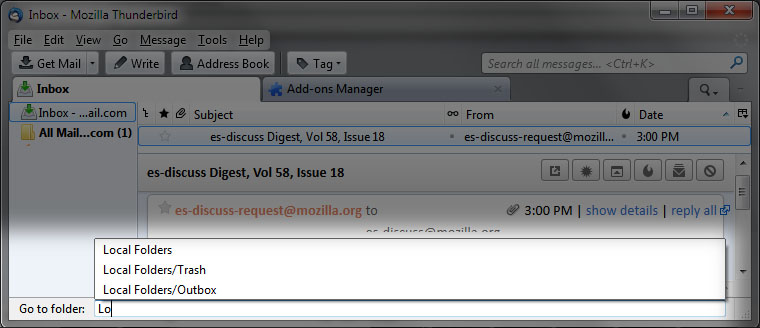
\includegraphics[width=\columnwidth]{nostalgy}
  \caption{Nostalgy's main interface: a folder selector in the status
    bar}
  \label{fig:nostalgy-screenshot}
\end{figure}
\begin{figure}
  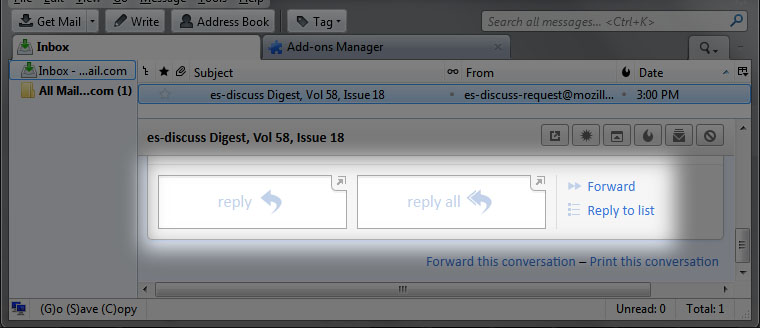
\includegraphics[width=\columnwidth]{conversations}
  \caption{Thunderbird Conversation's main interface: text boxes in
    the conversation view for quick replies}
  \label{fig:conversation-screenshot}
\end{figure}
One of the present authors routinely uses several extensions to
customize Thunderbird.  One such extension is Nostalgy~[CITE], which
provides several convenient hot keys for archiving messages and
navigating among folders.  For example, pressing `S' will save the
current message.  This is achieved by two event listeners on
the Thunderbird global \impl{window} object:

\begin{alltt}
function onNostalgyKeyPressCapture(event) \{
  // handle ESC key
  // handle Nostalgy cancellation
\}
function onNostalgyKeyPress(event) \{
  // show folder selector
  // handle key commands
\}
window.addEventListener("keypress", 
          onNostalgyKeyPress, false);
window.addEventListener("keypress", 
          onNostalgyKeyPressCapture, true);
\end{alltt}

Implicit in this code is the assumption that all keypresses are
intended to control Thunderbird, and not, for example, to input text.
However, another extension allows the user to do just that.
Thunderbird Conversations~[CITE] redefines the email preview pane to
show a Gmail-like conversation view, complete with ``quick reply''
boxes where the user can compose a response without leaving the main
window.  This functionality is implemented by the default actions of
the quick-reply \stag{textarea} tags, along with a bubble-phase
listener on their grandparent \stag{div}:
\begin{alltt}
quickReplyDiv.addEventListener("keydown", 
  function convKeyDown(event) \{
    // If ENTER then send message
    // If ESC then cancel editing
    event.stopPropagation();
  \});
\end{alltt}

At first glance, nothing in this code appears problematic; indeed,
Conversations and Nostalgy are listening to two different events.
However, our model includes the fact that the default action of a
``keydown'' event is to dispatch a ``keypress'' event, and while
Conversations does \impl{stopPropagation}, it does not
\impl{preventDefault}---which means that any key strokes typed into
the quick-reply box will effectively call \impl{convKeyDown},
\impl{onNostalgyKeyPressCapture} and finally
\impl{onNostalgyKeyPress}.  Consequently, typing a word containing an
`S' will steal focus from editing the message, and jump to Nostalgy's
``Save Message'' UI!  And indeed, if we input the Thunderbird DOM and
these three event listeners into our model, it confirms that this
behavior is correct according to the event dispatch rules.

When the author contacted the developers of 
Conversations, he implemented the following fix:
\begin{alltt}
quickReplyDiv.addEventListener("keypress",
  function convKeyPress(event) 
    \{ event.stopPropagation(); \});
quickReplyDiv.addEventListener("keyup",
  function convKeyUp(event)
    \{ event.stopPropagation(); \});
\end{alltt}
Adding these two listeners to our model shows that event dispatch now
calls \impl{convKeyDown}, \impl{onNostalgyKeyPressCapture}, and
\impl{convKeyPress}, and no longer calls \impl{onNostalgyKeyPress},
thereby avoiding the bug for now.  However, some of Nostalgy's code
still gets called, leaving open the potential for future bugs.  A
simpler, and more robust, fix is available: adding a call to
\impl{preventDefault} in \impl{convKeyDown} would prevent the
dispatch of the ``keypress'' event in the first place.

Generalizing from this example, we can annotate listeners in our model
with provenance information, and then query the model whether there
exist any $(\mathit{eventType}, \mathit{targetNode})$ pairs for which
dispatch will cause control to flow from one extension's listeners to
another's.  We anticipate that such queries will statically yield
other pairs of extensions whose behavior might conflict; for example,
the Conversations author knows it is incompatible with other hot-key
related extensions, and this analysis can determine others, or help
pinpoint where bugfixes are needed.

\section{Conclusion}\label{sec:conclusion}
\lipsum[1]

%\appendix
%\section{Appendix Title}
%
%This is the text of the appendix, if you need one.
%

%\acks
%
%Acknowledgments, if needed.
%

{\footnotesize \bibliographystyle{acm}
\bibliography{safebrowser}
\lipsum[1-3]}

\theendnotes

\end{document}

